\documentclass[11pt,a4paper]{article}
\usepackage[margin=2cm]{geometry}
\usepackage[T1]{fontenc}
\usepackage{mathptmx}
\usepackage{amsmath,amssymb}
\usepackage{graphicx}
\usepackage{xcolor}
\usepackage{enumitem}
\usepackage{array}
\usepackage{float}
\usepackage{colortbl}
\usepackage{needspace}
\usepackage[labelformat=empty,skip=4pt]{caption}
\usepackage[hidelinks]{hyperref}
\graphicspath{{figs/}}
\definecolor{navy}{HTML}{1B3755}
\definecolor{headc}{HTML}{E6ECF5}
\definecolor{okc}{HTML}{DFF3DF}
\definecolor{noc}{HTML}{FBE0E0}
\setlength{\parindent}{0pt}
\setlength{\parskip}{5pt}
\renewcommand{\arraystretch}{1.25}
\newcommand{\sect}[1]{\needspace{8\baselineskip}\bigskip{\Large\color{navy}\bfseries #1}\par\smallskip{\color{navy}\hrule height 0.8pt}\smallskip}
\newcommand{\sub}[1]{\needspace{5\baselineskip}\medskip{\large\color{navy}\bfseries #1}\par}
\newcommand{\slideline}[1]{\par\smallskip\noindent\fcolorbox{navy}{headc}{\parbox{\dimexpr\linewidth-2\fboxsep-2\fboxrule}{\textbf{What you say on the slide:} \emph{#1}}}\par}
\newcommand{\say}[1]{\par\smallskip\noindent\fbox{\parbox{\dimexpr\linewidth-2\fboxsep-2\fboxrule}{\textbf{In one sentence:} #1}}\par}
\newcommand{\q}[1]{\par\needspace{4\baselineskip}\medskip\noindent\textbf{Q.\ #1}\par\noindent}
\newcommand{\hd}{\rowcolor{headc}}

\begin{document}
\begin{center}
{\LARGE\bfseries\color{navy} Three Statements of the Presentation, Explained}\\[4pt]
{\large Zero margin and practical margin \;$\cdot$\; the 1896 times within 1.22 per cent \;$\cdot$\; the EMT result}\\[2pt]
IEEE 13-node feeder, DIgSILENT PowerFactory --- Jhala Nath Kafle (081MSPSE009)
\end{center}

% =====================================================================================================
\sect{Part A. Zero margin and practical margin}
\slideline{These counts use a zero margin; with a three-cycle breaker time they become 31, and 26 with a fuse
safety margin as well. (Slide 25; also the conclusion, slide 26.)}

\say{``Margin'' is how much earlier than the fuse the recloser must act before a fault is counted as
coordinated: with a zero margin ``earlier by any amount'' is enough (38 of 39 cells), and with a practical
margin the recloser must still be earlier after the breaker time and a fuse allowance are included (31, then
26 cells).}

\sub{A.1 The quantity}
For fuse saving the recloser must interrupt the fault before the fuse element starts to melt. The time
between the two is the coordination time interval:
\[
\mathrm{CTI} = t_{MMT}(I_{fuse}) - t_{fast}(I_{recloser})
\]
$t_{MMT}$ is the minimum-melting time of the fuse from its curve; $t_{fast}$ is the operating time of the
recloser's \emph{relay} from its fast curve. A cell is a node with a fault type; there are 39.

\sub{A.2 The three tests}
\begin{table}[H]\centering\small
\begin{tabular}{|p{3.3cm}|p{4.7cm}|p{5.2cm}|c|}\hline
\hd \textbf{Name} & \textbf{Test for ``held''} & \textbf{What it assumes} & \textbf{Cells held} \\ \hline
Zero margin & $t_{fast} < t_{MMT}$ \quad (CTI $>0$) & the breaker opens the instant the relay operates; the
fuse curve is exact & \cellcolor{okc}38 of 39 \\ \hline
Breaker time & $t_{fast} + 0.050\,\text{s} < t_{MMT}$ & the breaker needs 3 cycles (0.050\,s at 60\,Hz) to
interrupt the current & 31 of 39 \\ \hline
Breaker time and fuse allowance & $t_{fast} + 0.050\,\text{s} < 0.75\,t_{MMT}$ & in addition, the fuse is only
loaded to 75\,\% of its melting time (tolerance, pre-loading, ageing) & 26 of 39 \\ \hline
\end{tabular}
\end{table}
All three use the \textbf{same fault currents, the same settings (DSDR) and the same revised fuses}, with the DG
in service. Nothing is simulated again: only the test changes. The other conditions (fuse clears before the
delayed trip, series fuses, R2 against R1) are the same in all three.

\begin{figure}[H]\centering
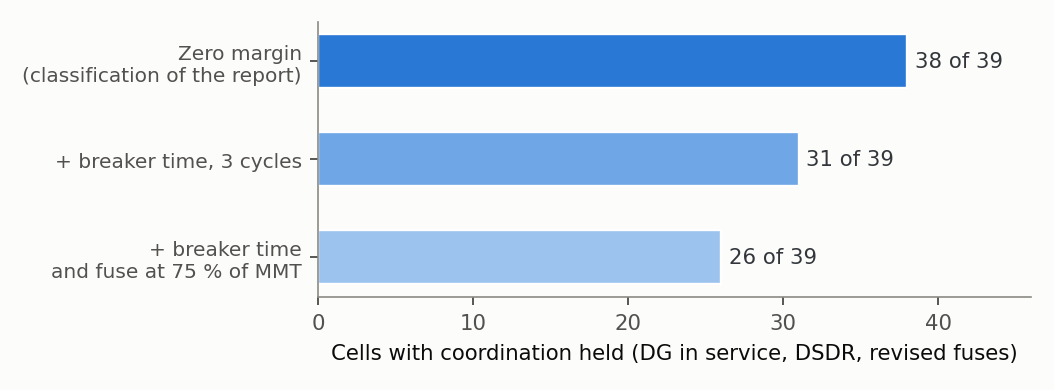
\includegraphics[width=0.74\textwidth]{margin_counts.png}
\end{figure}

\sub{A.3 Three faults that show the difference}
\begin{figure}[H]\centering
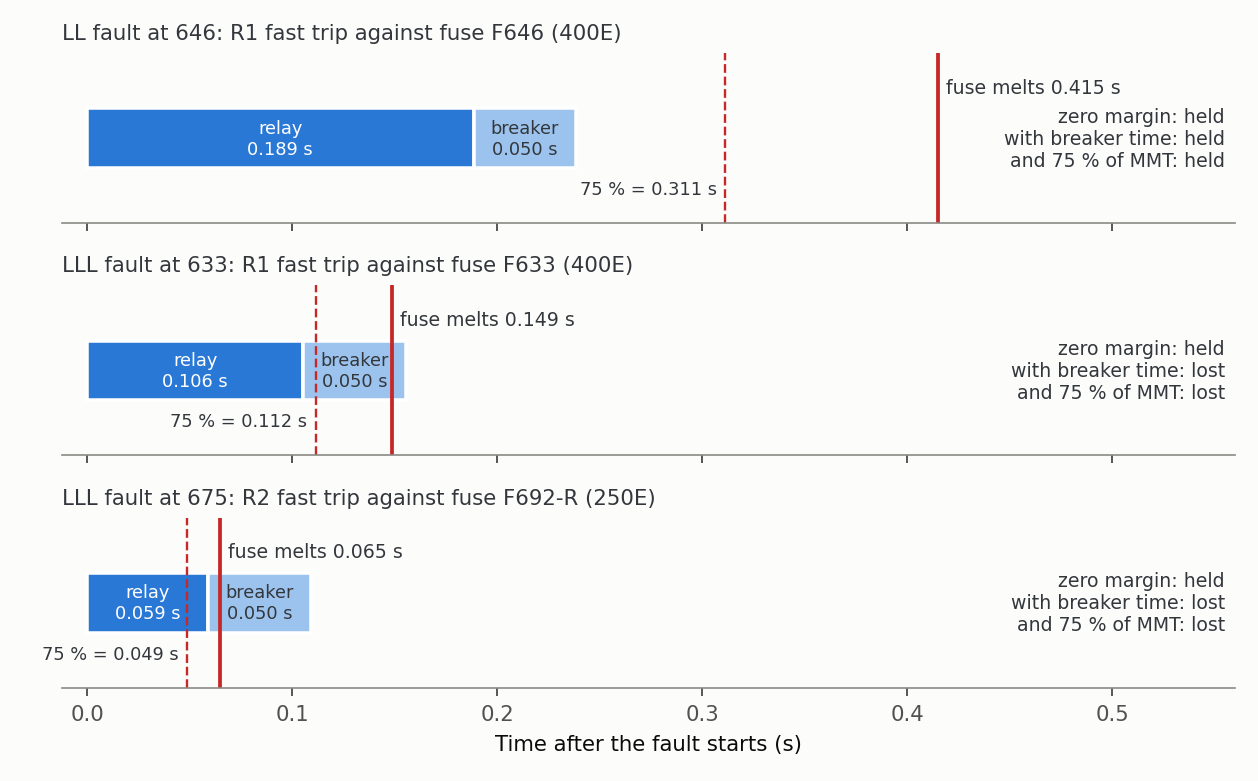
\includegraphics[width=0.92\textwidth]{margin_cases.png}
\caption{\small The blue bar is the relay time on its fast curve; the light bar is the breaker time. Solid red
line: the fuse starts to melt. Dashed red line: 75\,\% of that time.}
\end{figure}
\begin{itemize}[leftmargin=*,itemsep=2pt]
\item \textbf{646, LL:} relay 0.189\,s, fuse 0.415\,s. The CTI is 226\,ms. Adding 50\,ms leaves 176\,ms, and
$0.239 < 0.311$: held in all three tests. A comfortable cell.
\item \textbf{633, LLL:} relay 0.106\,s, fuse 0.149\,s. The CTI is $+43$\,ms, so it is held with zero margin.
With the breaker, $0.106 + 0.050 = 0.156\,\text{s} > 0.149$\,s: the fuse has already started to melt when the
current is interrupted. Lost.
\item \textbf{675, LLL:} relay 0.059\,s, fuse 0.065\,s. The CTI is only $+6$\,ms (the smallest of the study).
Held with zero margin, lost with any practical margin.
\end{itemize}

\sub{A.4 Which cells change}
\begin{table}[H]\centering\small
\begin{tabular}{|p{5.2cm}|p{10.2cm}|}\hline
\hd \textbf{Step} & \textbf{Cells that are lost at this step} \\ \hline
Zero margin: 38 held & 692 LG (the only lost cell; limited by R2's delayed dial, not by the margin) \\ \hline
Add the breaker time: 31 held & 633 LLL; 675 LL, LLG, LLL; DL LLG, LLL; 652 LG \quad (7 cells) \\ \hline
Add the 75\,\% fuse allowance: 26 held & 633 LL, LLG; 684 LL, LLG; DL LL \quad (5 more cells) \\ \hline
\end{tabular}
\end{table}
The cells that go first are those near the DG and at the nodes with the highest fault current (633, 675, the
distributed load): there the fuse melts in about 0.1\,s, so 50\,ms of breaker time is a large part of it.

\sub{A.5 Where it was evaluated}
\begin{itemize}[leftmargin=*,itemsep=2pt]
\item \textbf{Report:} Section 5.15, ``Sensitivity of the Result to the Margin''. It is also stated in the
abstract, in the limitations (Section 1.6), in the coordination criteria (Section 3.8, which defines the zero
margin) and in the conclusion.
\item \textbf{Presentation:} slide 6 (limitation), slide 25 (summary) and slide 26 (conclusion).
\item \textbf{EMT run:} the only place where the breaker time is actually \emph{in} the simulation --- every
recloser trip there is the relay time plus 3 cycles.
\end{itemize}

\sub{A.6 Why the report classifies with a zero margin}
\begin{enumerate}[leftmargin=*,itemsep=2pt]
\item It is the criterion of the method being implemented: the fuse must not melt before the fast operation,
i.e.\ CTI $>0$. Using the same criterion keeps the result comparable with the reference.
\item It isolates the question the project asks: \emph{does the dual setting restore the order of
operation?} A margin is a second, separate question about how much reserve there is.
\item It does not hide anything: the effect of a practical margin is evaluated and reported next to it.
\end{enumerate}

\sub{A.7 How to defend it}
\q{Is a zero margin realistic?}
No, and I say so. It is the criterion of the method, used to compare like with like. That is why I also
evaluated a practical margin: with a three-cycle breaker time 31 cells are held, and with a fuse allowance as
well, 26. I report all three numbers.

\q{So your real result is 26, not 38?}
The three numbers answer three questions. 38 says the DSDR with the revised fuses restores the correct order
of operation in all cells but one. 31 and 26 say how many of those also have enough reserve for a real
breaker and a real fuse. The cells that drop out have a fuse that melts in about a tenth of a second; they
need a larger fuse or a faster recloser, not a different direction logic.

\q{Why three cycles? Why 75 per cent?}
Three cycles is a typical interrupting time of a recloser breaker; it is the value also used in the EMT run.
75 per cent of the minimum-melting time is the usual allowance for fuse tolerance, pre-loading and ageing,
and it is the same factor the method uses between series fuses.

\q{How would you improve the 26?}
The dials cannot go lower: R1 and R2 are already at their fastest settings. The remaining ways are larger or
slower fuses at 633, 675 and the distributed load (checked again for selectivity), a relay with a faster fast
curve, or a faster breaker. This is listed as future work: a classification with a practical margin.

\q{Does the margin change the comparison between single and dual setting?}
No. The margin shifts every case by the same test. The dual setting restores cells by making R2 trip on its
reverse group; whether there is 50\,ms of reserve after that depends on the fuse.

% =====================================================================================================
\newpage
\sect{Part B. ``PowerFactory's own relay models confirm all 1896 times within 1.22 per cent''}
\slideline{It is checked twice: R1 reproduces the paper's worked example, and PowerFactory's own relay models
confirm all 1896 times within 1.22 per cent. (Slide 9; also slides 25 and 26.)}

\say{Every operating time in the study was obtained twice --- once by my calculation from the device curves,
once by PowerFactory's built-in relay and fuse elements with the same settings --- and in 1896 comparisons the
two never differ by more than 1.22 per cent.}

\sub{B.1 What was compared}
\begin{itemize}[leftmargin=*,itemsep=2pt]
\item \textbf{Method 1, the calculation.} The operating times of Chapter Five are calculated from the
time--current curves of the devices (the IAC equation for R1, the CDG34 table for R2, the A055C curves for
the fuses), using the currents of the PowerFactory short-circuit study.
\item \textbf{Method 2, PowerFactory itself.} The same settings were entered into the relay and fuse
\emph{elements} of the model. For each fault, PowerFactory then reports the tripping time of every device.
\item \textbf{The comparison.} For each device and each fault, the difference between the two times in per
cent. In the report this is Section 5.14, ``Verification With the Relay and Fuse Models of PowerFactory''.
\end{itemize}

\sub{B.2 Where the number 1896 comes from}
One comparison is one device for one fault.
\begin{table}[H]\centering\small
\begin{tabular}{|p{6.4cm}|c|p{6.2cm}|}\hline
\hd \textbf{How the 1896 are made up} & \textbf{Number} & \textbf{Note} \\ \hline
Conventional settings & 780 & R1 and R2, fast and delayed; the fuses \\ \hline
DSDR settings & 1116 & also the reverse group of R2, fast and delayed \\ \hline
\hd Total & 1896 & \\ \hline
DG out of service / DG in service & 948 / 948 & \\ \hline
R1 / R2 / fuses & 672 / 1008 / 216 & \\ \hline
Faults & & 12 nodes; LG, LL, LLG and LLL; every phase combination that exists at the node \\ \hline
\end{tabular}
\end{table}
\textbf{Be exact about one detail:} in 1647 of the 1896 comparisons the device operates and two \emph{times} are
compared. In the other 249 the current is below the pickup, and both methods say ``no trip''. They agree in all
249. So the accurate statement is: 1896 comparisons, of which 1647 are operating times, all within 1.22 per
cent, and 249 are no-trip cases that agree.

\sub{B.3 How close they are}
\begin{figure}[H]\centering
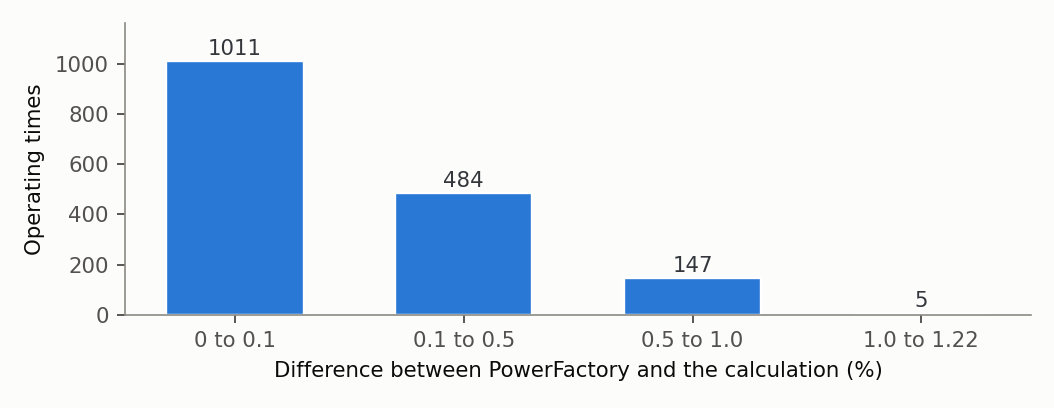
\includegraphics[width=0.66\textwidth]{pf_check.png}
\caption{\small The 1647 operating times, by the size of the difference.}
\end{figure}
\begin{table}[H]\centering\small
\begin{tabular}{|p{7cm}|p{8.2cm}|}\hline
\hd \textbf{Quantity} & \textbf{Value} \\ \hline
Largest difference & 1.22\,\% \\ \hline
Where & LG fault at 645, phase c, DG in, R2 reverse group, fast: PowerFactory 0.3373\,s, calculation
0.3415\,s --- 4\,ms \\ \hline
Average difference & 0.15\,\% \\ \hline
Half of the times differ by less than & 0.03\,\% \\ \hline
1\,\% or more & 5 times, all on the fast curve of R2's reverse group \\ \hline
R1 (equation) & identical in all 672 comparisons \\ \hline
Fuses & at most 0.46\,\% \\ \hline
\end{tabular}
\end{table}

\sub{B.4 Why they are not exactly equal}
R1 follows an equation, so the two methods agree to the last digit. R2 follows a \textbf{table} of points given
by the manufacturer. Between two points the time has to be interpolated, and my interpolation (straight lines on
log-log axes) is not identical to PowerFactory's. The largest differences are where the curve bends most, at
low multiples of the plug setting; all five differences of 1\,\% or more are on the fast curve of the reverse
group.

\sub{B.5 What the check proves, and what it does not}
\begin{table}[H]\centering\small
\begin{tabular}{|p{7.5cm}|p{7.9cm}|}\hline
\hd \textbf{It proves} & \textbf{It does not prove} \\ \hline
The curves were implemented correctly: equation, constants, table, interpolation, CT ratios, plug and dial &
That the fault currents are right --- both methods use the same PowerFactory currents. That is checked
separately against the IEEE benchmark (within about 2\,\%) \\ \hline
The settings in the model are the settings in the report & That the chosen settings are the best ones \\ \hline
The classification (held / lost) does not depend on my own calculation: an independent tool gives the same
times & That real devices behave exactly like their published curves \\ \hline
\end{tabular}
\end{table}

\sub{B.6 How to defend it}
\q{What does ``1896 times within 1.22 per cent'' mean?}
Every operating time of the study was obtained twice: by my calculation from the manufacturers' curves, and
by PowerFactory's own relay and fuse elements with the same settings. That gives 1896 comparisons over all
nodes, fault types, phase combinations, DG in and out, and both schemes. The largest difference is 1.22 per
cent, which is 4 milliseconds.

\q{Why calculate the times yourself if PowerFactory can do it?}
To make every number traceable: each time in the report can be followed back to a curve, a current and a
setting, and the dual setting --- two groups selected by direction --- is not a function of the library relay.
PowerFactory's own elements were then used as an independent check of that calculation.

\q{Is 1.22 per cent acceptable?}
Yes. It is 4 milliseconds on a time of 0.34 seconds. Relay timing tolerances are several per cent, and fuse
curves have a tolerance of about ten per cent. The average difference is 0.15 per cent.

\q{Where does the difference come from?}
From interpolation in the CDG34 table. R1 is an equation and agrees exactly. R2 is a table of points; between
the points I interpolate on log-log axes and PowerFactory interpolates in its own way.

\q{Does this prove your results are correct?}
It proves the curves and settings are implemented correctly. The fault currents are a separate matter, and I
checked those against the IEEE short-circuit benchmark. Together: the currents are right within about 2 per
cent, and the times from those currents are right within 1.22 per cent.

\q{Could the difference change a held cell to lost?}
Only where the CTI is smaller than the difference. The smallest CTI is 6\,ms at 675, on R2's \emph{forward}
group at a high current, where the two methods differ by 0.1\,ms (0.0590 against 0.0591\,s). The 4\,ms difference is
on the reverse group at 645, where the CTI is 1.4 seconds.

% =====================================================================================================
\newpage
\sect{Part C. The EMT statement}
\slideline{This EMT simulation is a line-to-line fault at 684. Without DG, the two fast shots use only 45 per
cent of the fuse's melting heat, and the fuse then clears the permanent fault. With the DG, current keeps
flowing while R2 is open, and the fuse melts at 0.75 seconds, during the second fast shot. (Slide 23.)}

\say{The EMT run follows one fault through the whole reclosing sequence in time, and shows that the fuse
survives the two fast shots without DG but not with DG.}

\sub{C.1 The statement, piece by piece}
\begin{table}[H]\centering\small
\begin{tabular}{|p{4.6cm}|p{10.8cm}|}\hline
\hd \textbf{Words} & \textbf{Meaning} \\ \hline
``EMT simulation'' & A time-domain simulation: PowerFactory solves the network every 0.1\,ms and gives the
current \emph{wave}, not one RMS number. It can include breakers opening and reclosing. \\ \hline
``line-to-line fault at 684'' & Phases a--c at node 684 through 0.2\,$\Omega$, starting at 0.30\,s; permanent.
684 is downstream of R2; the fuse F671-2 (300E) protects that lateral; the DG at 692 sits between R2 and the
fuse. \\ \hline
``the two fast shots'' & R2 trips on its fast curve, waits 0.2\,s (dead time), recloses, and trips on the
fast curve again. Each shot lasts 0.120\,s: 0.070\,s relay time + 0.050\,s breaker time. \\ \hline
``use only 45 per cent of the fuse's melting heat'' & A fuse melts when it has absorbed enough heat. Each
instant of current uses a fraction $\Delta t / t_{MMT}(I)$ of it. Without DG the fuse carries 2441\,A, where
it needs 0.553\,s to melt. Two shots of 0.120\,s: $2 \times 0.120 / 0.553 \approx 45\,\%$. The fuse is intact. \\ \hline
``the fuse then clears the permanent fault'' & The fault is still there after the second reclose. R2 is now on
its delayed curve (2.67\,s), so the fuse melts first, at 1.248\,s, and has cleared at 1.613\,s. Only the
faulted lateral is lost. This is the intended fuse-saving sequence. \\ \hline
``With the DG, current keeps flowing while R2 is open'' & When R2 opens, the grid is cut off, but the DG is
still connected to the fault through the fuse. About 1230\,A flows during the dead time, so the fuse keeps
heating. Without DG that current is zero. \\ \hline
``the fuse melts at 0.75 seconds, during the second fast shot'' & With DG the fuse carries 4322\,A (grid +
DG) instead of 2816\,A, and reaches 100\,\% of its melting heat at 0.752\,s --- one millisecond before R2's
second trip at 0.753\,s. Fuse saving is lost: a temporary fault would cost a fuse. \\ \hline
\end{tabular}
\end{table}

\begin{figure}[H]\centering
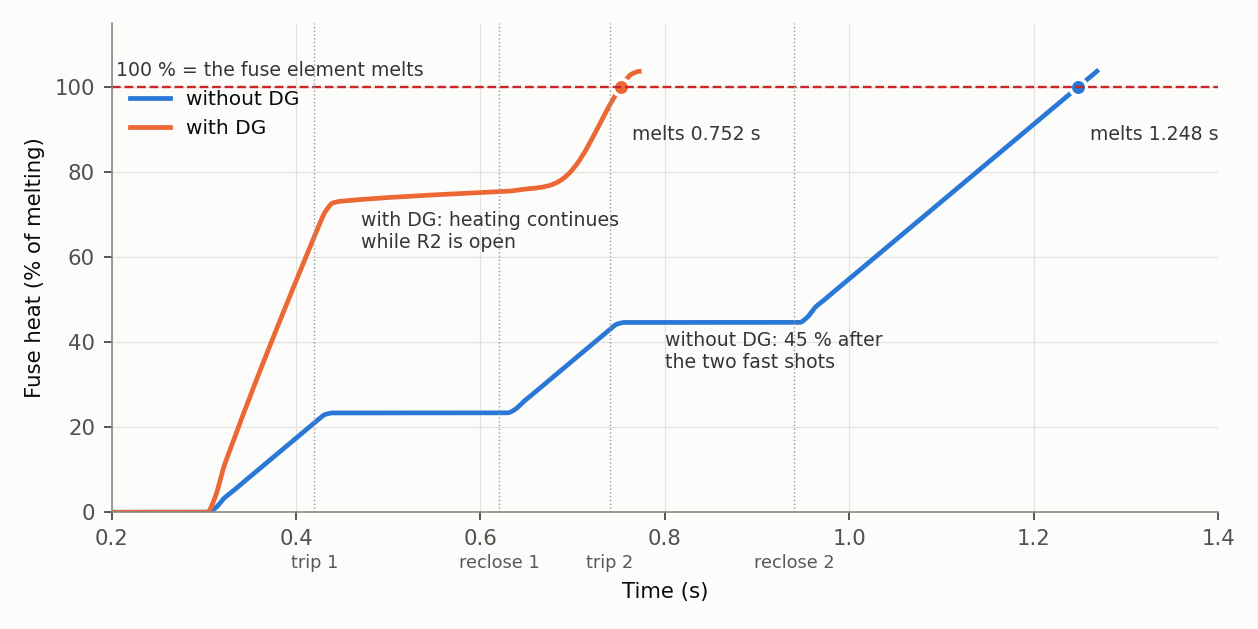
\includegraphics[width=0.80\textwidth]{emt_heat.png}
\caption{\small Fuse heat against time. Flat parts: no heating. The orange line keeps rising while R2 is open.}
\end{figure}

\sub{C.2 The heat budget}
\begin{table}[H]\centering\small
\begin{tabular}{|p{5cm}|c|c|c|c|}\hline
\hd & \multicolumn{2}{c|}{\textbf{Without DG}} & \multicolumn{2}{c|}{\textbf{With DG}} \\ \hline
\hd \textbf{Interval} & \textbf{added} & \textbf{total} & \textbf{added} & \textbf{total} \\ \hline
Fast shot 1 & 21\,\% & 21\,\% & 68\,\% & 68\,\% \\ \hline
Dead time 1 (R2 open) & 2\,\% & 23\,\% & 7\,\% & 75\,\% \\ \hline
Fast shot 2 & 20\,\% & 43\,\% & 25\,\% & \cellcolor{noc}100\,\% \\ \hline
Dead time 2 (R2 open) & 2\,\% & \cellcolor{okc}45\,\% & 5\,\% & 105\,\% \\ \hline
\end{tabular}
\end{table}

\sub{C.3 Why the fuse melts with DG --- three reasons}
\begin{enumerate}[leftmargin=*,itemsep=2pt]
\item The fuse carries more current: 4322\,A against 2816\,A. One shot costs 68\,\% instead of 21\,\%.
\item R2 sees less and is slower: 2436\,A against 2607\,A, so its shot lasts 0.126\,s instead of 0.120\,s.
\item The DG keeps feeding the fault in the dead time: about 1230\,A, adding 7\,\% and 5\,\%.
\end{enumerate}

\begin{figure}[H]\centering
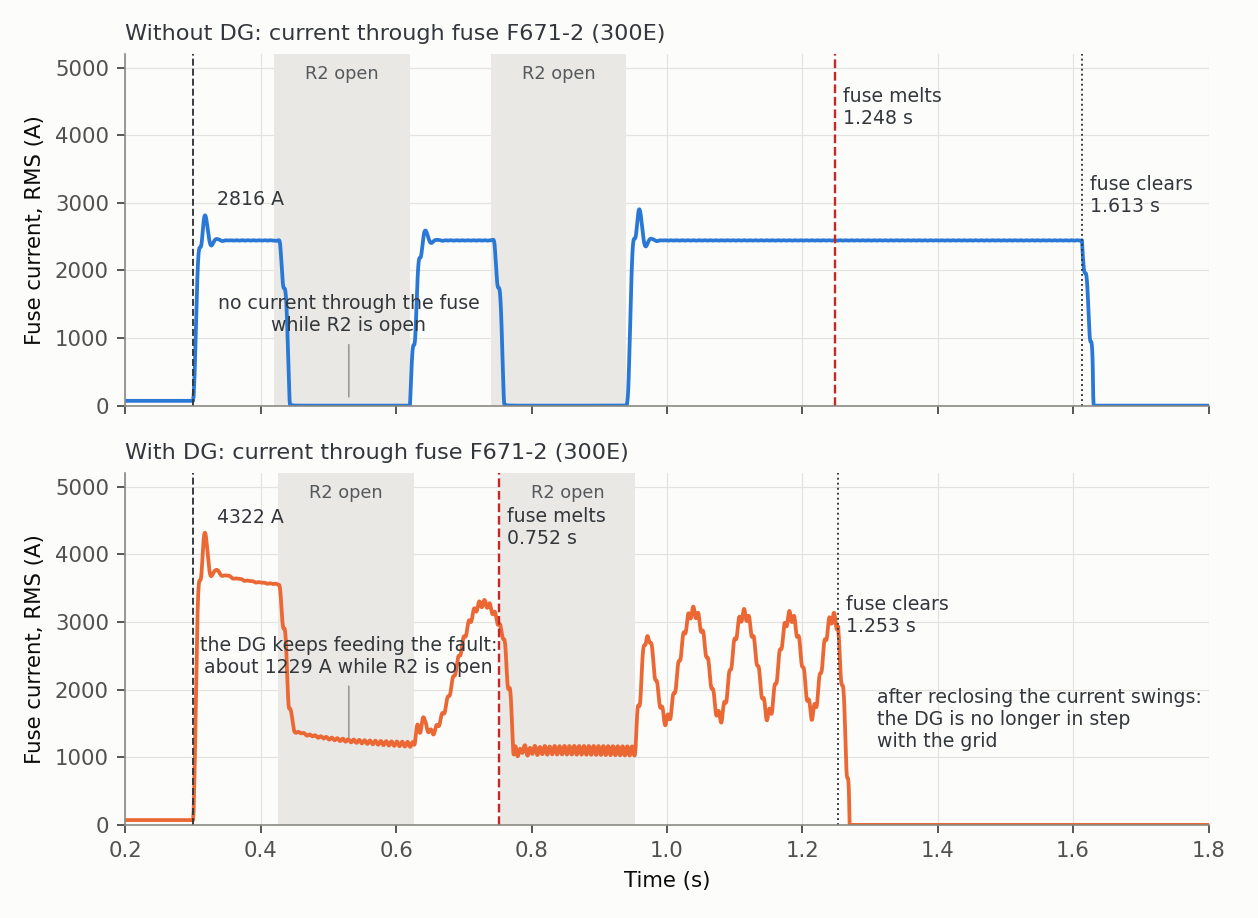
\includegraphics[width=0.82\textwidth]{emt_sequence.png}
\caption{\small RMS current through the fuse. Grey: R2 open. With DG (below) the current does not fall to zero.}
\end{figure}

\sub{C.4 How to defend it}
\q{Why an EMT run when you already have the classification?}
The classification checks one fast trip against the fuse. A reclosing sequence has two fast shots and dead
times, and the fuse heat adds up. Only a time-domain run shows that, and shows what the DG does while the
recloser is open.

\q{How do you get 45 per cent?}
Without DG the fuse carries about 2441 amperes, where it needs 0.553 seconds to melt. Each fast shot lasts
0.120 seconds, about 22 per cent each, so two shots use about 45 per cent.

\q{The fuse blows at 1.25 seconds even without DG. Is that a failure?}
No. The fault is permanent. The fast shots give a temporary fault two chances; when it is still there, R2
goes to its delayed curve and the fuse clears its own lateral. That is correct fuse saving.

\q{Why conventional settings and not the DSDR?}
The fault at 684 is downstream of R2. There R2 carries forward current in both schemes and its forward group
is the same, so the sequence would be identical. For faults downstream of R2 the DG feeds the fault directly;
no setting of R2 changes that. It is the limit stated in the conclusion.

\q{How do you know the EMT is right?}
The fuse carried fault current for $0.120 + 0.120 + 0.308 = 0.548$ seconds before melting, and its curve
gives 0.553 seconds at that current. The peak of the wave over its RMS value is $\sqrt{2}$.

\q{In practice the DG protection would trip the DG.}
The DG protection is not modelled, and I state that. If the DG tripped in the first dead time, the dead-time
infeed would disappear. But the first shot would still use 68 per cent instead of 21, because that happens
before any DG protection can act.

\medskip
{\small The full account of the EMT run, with more figures and 26 questions, is in
\texttt{DSDR\_EMT\_Guide.pdf}.}

\end{document}
